 \begin{enumerate}
	 \item The volume of a conical tent is $462 m^{3}$ and the area of the base is $154 m^{2}$. The height of the cone is:
		 \begin{enumerate}
			 \item $15 m$
			 \item $12 m$
			 \item $9 m$
			 \item $24 m$
		 \end{enumerate}
	 \item The radius of a roller $100 cm$ long is $14 cm$. The curved surface area of the roller is: $(Take \pi = \frac{22}{7})$
		 \begin{enumerate}
			 \item $13200 cm^{2}$
			 \item $15400 cm^{2}$
			 \item $4400 cm^{2}$
			 \item $8800 cm^{2}$
		 \end{enumerate}
	 \item A solid cone of radius $5 cm$ and height $9 cm$ is melted and made into small cyliders of radius of $0.5 cm$ and height $1.5 cm$. Find the number of cylinders so formed.
	 \item A solid wooden cylinder is of radius $6 cm$ and height $16 cm$. Two cones ech of radius $2 cm$ and height $6 cm$ are drilled out of the cylinder. Find the volume of the remainiing solid.\\
		 \begin{figure}[h]
			 \centering
			 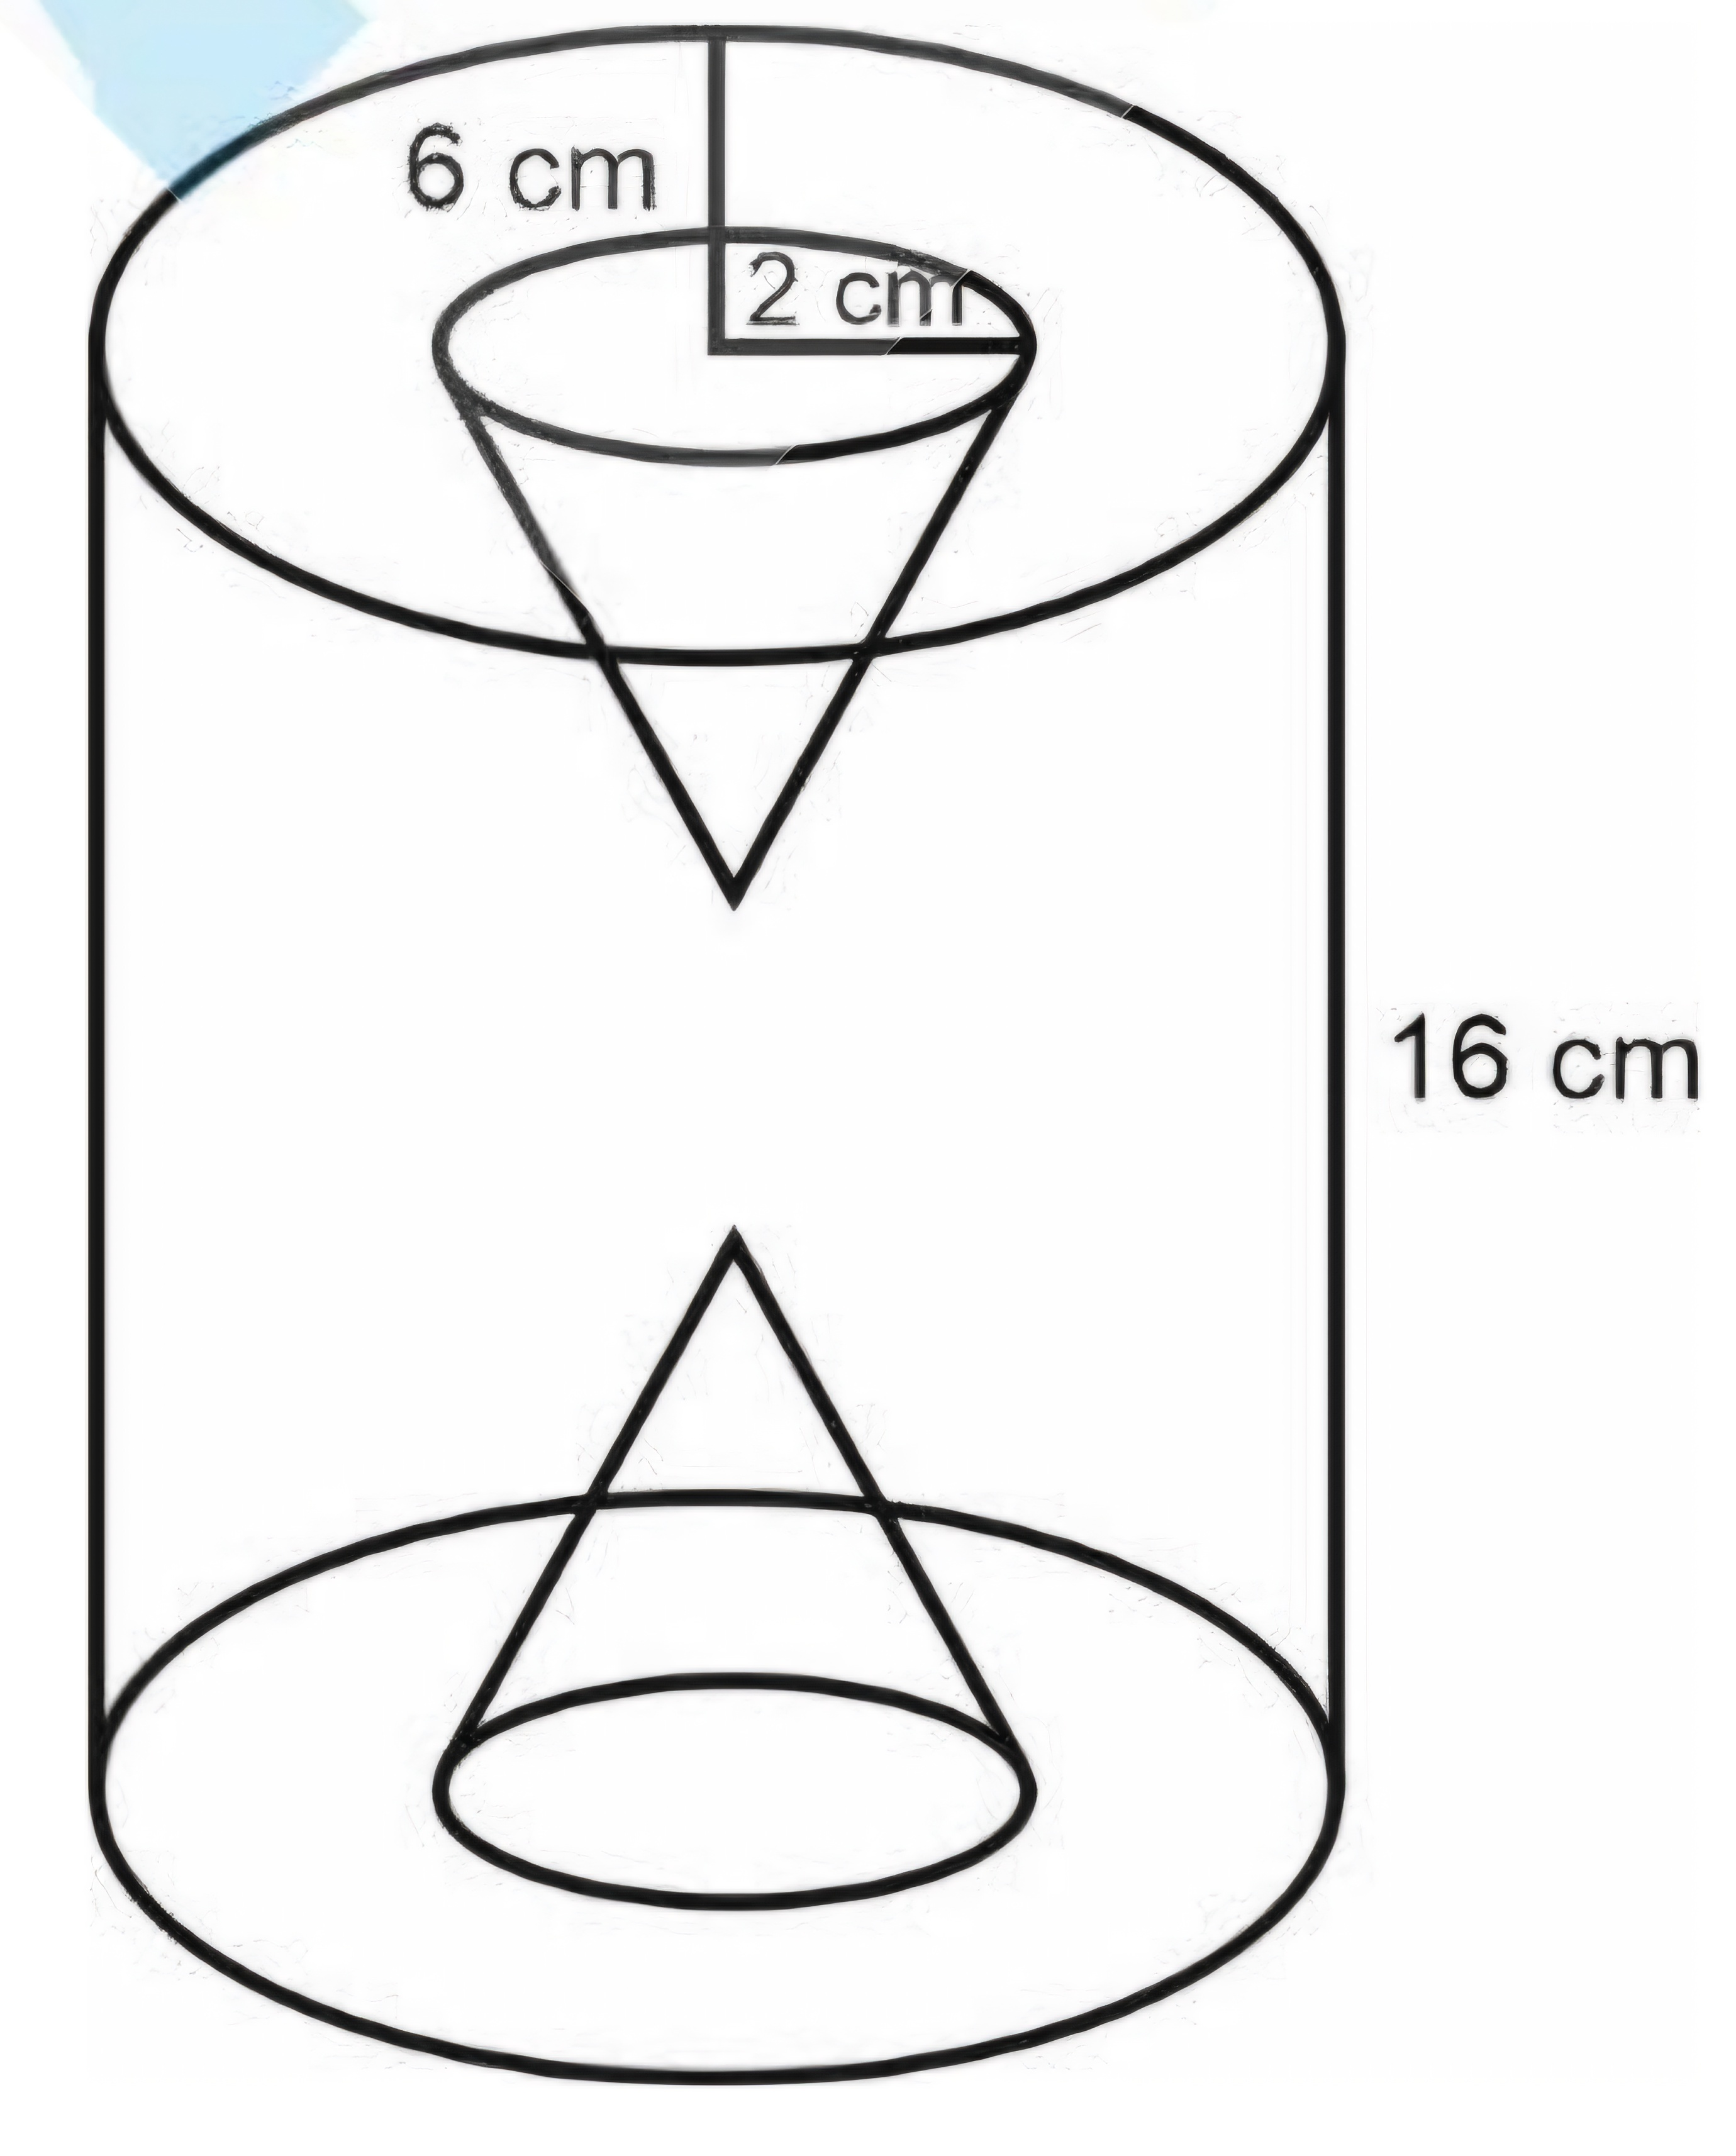
\includegraphics[width=\columnwidth]{figs/img1.jpg}
			 \caption{}
			 \label{Figure}
		 \end{figure}
 \end{enumerate}
